%%%%%%%%%%%%%%%%%%%%%%%%%%%%%%%%%%%%%%%%%
% University Assignment Title Page 
% LaTeX Template
% Version 1.0 (27/12/12)
%
% This template has been downloaded from:
% http://www.LaTeXTemplates.com
%
% Original author:
% WikiBooks (http://en.wikibooks.org/wiki/LaTeX/Title_Creation)
%
% License:
% CC BY-NC-SA 3.0 (http://creativecommons.org/licenses/by-nc-sa/3.0/)
%
%%%%%%%%%%%%%%%%%%%%%%%%%%%%%%%%%%%%%%%%%
%\title{Title page with logo}
%----------------------------------------------------------------------------------------
%	PACKAGES AND OTHER DOCUMENT CONFIGURATIONS
%----------------------------------------------------------------------------------------

\documentclass[12pt]{article}
\usepackage[english]{babel}
\usepackage[utf8]{inputenc}
\usepackage{natbib}
\usepackage{amsmath}
\usepackage{color}
\usepackage[explicit]{titlesec}
\usepackage[hyphens,spaces,obeyspaces]{url}
\usepackage{graphicx}
\usepackage{caption}
\usepackage{subcaption}
\usepackage{grffile}
\usepackage{listings}
\usepackage{placeins}

\usepackage{booktabs}
\usepackage{tabularx}

\begin{document}

\begin{titlepage}

\newcommand{\HRule}{\rule{\linewidth}{0.5mm}} % Defines a new command for the horizontal lines, change thickness here

\center % Center everything on the page
 
%----------------------------------------------------------------------------------------
%	HEADING SECTIONS
%----------------------------------------------------------------------------------------

\textsc{\LARGE University of St Andrews}\\[1.5cm] % Name of your university/college
\textsc{\Large Distributed Systems}\\[0.5cm] % Major heading such as course name
\textsc{\large CS4103}\\[0.5cm] % Minor heading such as course title

%----------------------------------------------------------------------------------------
%	TITLE SECTION
%----------------------------------------------------------------------------------------

\HRule \\[0.4cm]
{ \huge \bfseries Ring-Based Distributed System}\\[0.4cm] % Title of your document
\HRule \\[1.5cm]
 
%----------------------------------------------------------------------------------------
%	AUTHOR SECTION
%----------------------------------------------------------------------------------------


\Large \emph{Author:}\\
 \textsc{150008022}\\[1cm] % Your name
 
%----------------------------------------------------------------------------------------
%	DATE SECTION
%----------------------------------------------------------------------------------------

{\large \today}\\[2cm] % Date, change the \today to a set date if you want to be precise

%----------------------------------------------------------------------------------------
%	LOGO SECTION
%---------------------------------------------------------------------------------------


\includegraphics[width = 4cm]{images/standrewslogo.png}
 
%----------------------------------------------------------------------------------------

\vfill % Fill the rest of the page with whitespace

\end{titlepage}

\section*{Goal}

To demonstrate an understanding of leader election and mutual exclusion in distributed systems by developing a ring-based distributed social media application.

\tableofcontents
\newpage

\pagenumbering{arabic}
\setcounter{page}{1} 

\section{Initial Set-up}

Java 8 was chosen for this project due to it's friendly socket API, and Maven \cite{maven} was used as the build tool. 

Since each node would be running on an isolated machine, the planned testing environment would involve using \emph{ssh} to start the nodes remotely. Providing the configuration as command line arguments was considered simpler than other methods, and was implemented using the Apache Commons CLI library \cite{apachecli}. In order to run the program, the arguments shown in table \ref{tbl:arguments} had to be specified. The purpose of each argument is explained later.

\renewcommand{\arraystretch}{1.5}
\begin{table}[!ht]
\centering
\begin{tabular}{ll}
\multicolumn{2}{l}{usage: java -jar $\langle$program$\rangle$.jar}
\\ 

 -d,--drop           &  Include if this node should trigger a database refresh. \\
 -e,--election $\langle$arg$\rangle$ &  Election method to use. \\
 -f,--list $\langle$arg$\rangle$     &  Path to file containing list of nodes (resource P). \\
 -i,--id $\langle$arg$\rangle$       &  ID of this node. 
\end{tabular}
\caption{Arguments for running application.}
\label{tbl:arguments}
\end{table}


\section{Ring Formation}

\subsection{Messages}

In order for nodes to understand and parse the node.nodemessaging that were sent between them, a message protocol was designed. Figure \ref{fig:mainmsg} shows the header that would be part of every message sent. The possible types of node.nodemessaging are summarised in table \ref{tbl:messagetypes}.

\begin{table}[!h]
\centering
\resizebox{\textwidth}{!}{%
\begin{tabular}{@{}lll@{}}
\toprule
Message Type                               & Usage                                                                                                                        & Payload                  \\ \midrule
\multicolumn{1}{l|}{JOIN}                  & \multicolumn{1}{l|}{Sent by new node to coordinator when wanting to join ring.}                                              & None                     \\
\multicolumn{1}{l|}{SUCCESSOR}             & \multicolumn{1}{l|}{Sent by coordinator to inform a node to connect to a new successor.}                                     & New Successor ID\\
\multicolumn{1}{l|}{SUCCESSOR\_REQUEST}    & \multicolumn{1}{l|}{Sent by a node to the coordinator after its successor has failed in order to be reassigned a successor.} & None                     \\
\multicolumn{1}{l|}{TOKEN}                 & \multicolumn{1}{l|}{Sent by a node to its successor.}                                                                        & None                     \\
\multicolumn{1}{l|}{TOKEN\_ACK}            & \multicolumn{1}{l|}{Sent by a node to its predecessor after receiving the token to confirm its reception.}                   & None                     \\
\multicolumn{1}{l|}{COORDINATOR\_ELECTION} & \multicolumn{1}{l|}{Message payload contains an election message.}                                                           & Election Message         \\ \bottomrule
\end{tabular}%
}
\caption{Possible values for the type field in the message header, with their usage and payload.}
\label{tbl:messagetypes}
\end{table}

The node.nodemessaging are sent as serialized Java objects, which requires that all message classes implement the \emph{Serializable} interface. A more platform independent format such as JSON would be preferred, but since all nodes would be using Java this method of serializing node.nodemessaging was kept. Figure \ref{fig:elecmsg} shows the header for an election message. The election message header would be in the payload of the main message. This allowed multiple election methods to be used and easy routing of election related node.nodemessaging to an election handler class.

\begin{figure}[!ht]
\centering
\begin{minipage}{.5\textwidth}
  \centering
  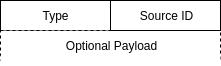
\includegraphics[width=.8\linewidth]{images/mainmsg}
  \captionof{figure}{Main message header.}
  \label{fig:mainmsg}
\end{minipage}%
\begin{minipage}{.5\textwidth}
  \centering
  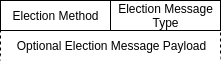
\includegraphics[width=.8\linewidth]{images/elecmsg}
  \captionof{figure}{Election message header.}
  \label{fig:elecmsg}
\end{minipage}
\end{figure}

\subsection{Transport Protocol}

Due to different patterns of communication during recovery and regular message passing phases both TCP and UDP were used for this project, as shown in Figure \ref{fig:pattern}.

\noindent \linebreak TCP was used for communication \textbf{around} the ring:
\begin{enumerate}
    \item Reliable communication avoids token being lost.
    \item Connection is reused frequently between predecessors and successors, justifying handshake overhead.
\end{enumerate}

\noindent UDP was used for communication \textbf{across} the ring: 
\begin{enumerate}
    \item Low communication overhead allows for node.nodemessaging to be sent to multiple nodes quickly, improving recovery time from node failure.
    \item No session maintenance allows coordinator to handle more members in the ring.
    \item Multicast communication possible which would greatly simplify broadcasting.
\end{enumerate}

\begin{figure}[!h]
\centering
\begin{subfigure}{.5\textwidth}
  \centering
  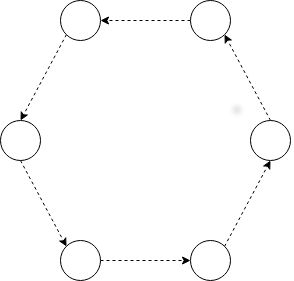
\includegraphics[width=.6\linewidth]{images/tcp}
  \caption{TCP Around Ring}
  \label{fig:tcp}
\end{subfigure}%
\begin{subfigure}{.5\textwidth}
  \centering
  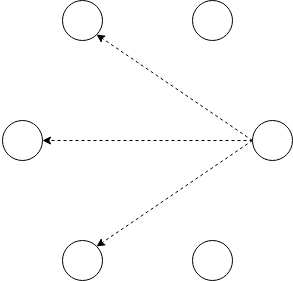
\includegraphics[width=.6\linewidth]{images/udp}
  \caption{UDP Across Ring}
  \label{fig:udp}
\end{subfigure}
\caption{The different types of communication used}
\label{fig:pattern}
\end{figure}

\subsection{Initialization and Joining}

On initialization, each node sends out join node.nodemessaging to the coordinator. The
joining protocol is similiar to that described in \cite{join}, and is shown in Figure \ref{fig:join}.
Figure \ref{fig:bigjoin} shows how the state of each connection changes over the course of
the joining procedure.

\begin{figure}[!ht]
\centering
  \centering
  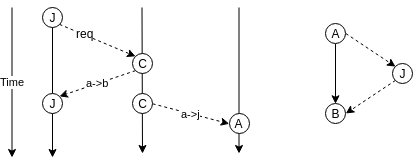
\includegraphics[width=.6\linewidth]{images/join}
  \caption{Joining protocol over time, with topology shown on right.}
\label{fig:join}
\end{figure}

\begin{figure}[!ht]
  \centering
  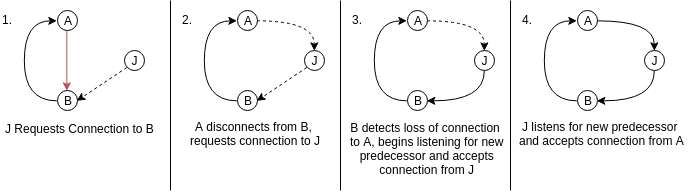
\includegraphics[width=\linewidth]{images/bigflow}
  \caption{State of each connection as a new node joins the ring. The red arrow
shows the edge that is replaced with the new node, and solid and dashed
arrows represent ongoing and pending connections respectively. Either A or
B can be the coordinator in this scenario.}
\label{fig:bigjoin}
\end{figure}
\FloatBarrier

\noindent When node J wants to join the ring:
\begin{enumerate}
    \item J sends join request to coordinator C.
    \item C sends successor to J, telling it to connect to B.
    \item C sends successor to A, telling it to connect to J. 
    \item A disconnects from B, B begins listening for new predecessor.
    \item J connects to B, A connects to J.
\end{enumerate}

In order for this process to work for a ring network with a single node,
it required another thread to wait on the connection, and the main thread
would then request the connection to itself. For two nodes and more the
joining node would be able to first connect to its new successor once its
predecessor had disconnected from its old successor as shown in figure \ref{fig:bigjoin}. 

Figure \ref{fig:succreq} shows the logs from node 2 as it joins the ring, and figure \ref{fig:succreqcoord} shows the logs from the coordinator as it handles the request. Figure \ref{fig:singlenodejoin} shows the logs from node 6 when it initializes the ring network by connecting to itself.

\begin{figure}[!ht]
	\centering
	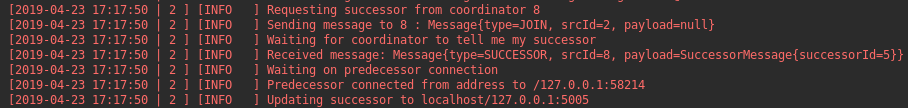
\includegraphics[width=\linewidth]{images/succreq}
	\caption{Logs from node 2 when joining the ring with coordinator ID 8.}
	\label{fig:succreq}
\end{figure}

\begin{figure}[!ht]
	\centering
	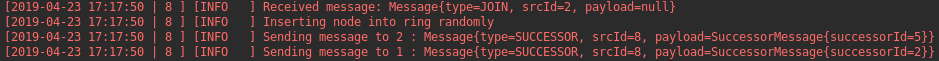
\includegraphics[width=\linewidth]{images/succreqcoord}
	\caption{Logs from coordinator node 8 when node 2 wishes to join.}
	\label{fig:succreqcoord}
\end{figure}

\begin{figure}[!ht]
	\centering
	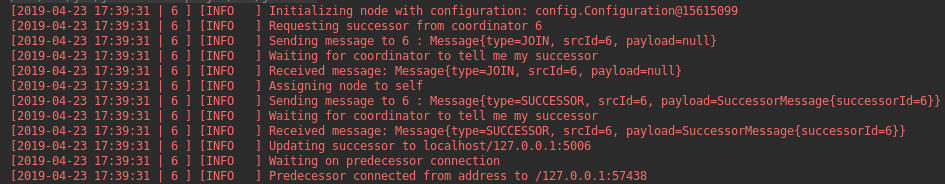
\includegraphics[width=\linewidth]{images/singlenodejoin}
	\caption{Logs from node 6 when it initializes the ring network and connects to itself.}
	\label{fig:singlenodejoin}
\end{figure}

\subsection{Topology Recovery and Maintenance}

When designing a distributed system, it should be assumed that failure will occur, and so as an extension this implementation included a mechanism for recovering from failure. Node failure is detected by either:
\begin{enumerate}
	\item a node attempting to read the socket connected to its predecessor.
	\item a node forwarding the token to its successor and not receiving an acknowledgement within a given timeframe.
\end{enumerate}

When a failure is detected by the successor of a failing node, it will simply begin listening for a new predecessor. Once the predecessor of the failing node detects the loss of connection, it will request a new successor from the coordinator node. The coordinator will then reply with the ID of the node after the failed node for the original predeccessor to connect to, at which point normal network behaviour can resume. Figure \ref{fig:failure} shows the topology change when a node fails. Since the failure is detected by the ring handling thread, and the new successor message arrives on the UDPSocket handling thread, the ring handling thread simply blocks until notified by the UDPSocket thread that a new successor has now been connected to. 

\begin{figure}[!ht]
	\centering
	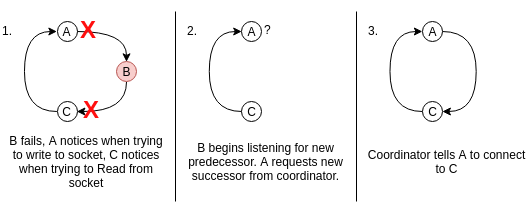
\includegraphics[width=\linewidth]{images/failure}
	\caption{Network topology during the recovery from node B failing. Either A or C are the coordinator in this scenario.}
	\label{fig:failure}
\end{figure}

The token acknowledgement message is the only occurence of communication in the reverse direction of the ring topology. The predecessor of the failing node will hold onto the token until it is assigned a new successor, and only releases the token once it has received the acknowlegement from it. This limits the number of situtations that can result in the loss of the token. If somehow the token is acknowledged but the acknowledgement message does not reach the predecessor in time, it could be possible for two tokens to then be in circulation. Figure \ref{fig:recovery} shows logs from a node that has experienced successor failure. 

\begin{figure}[!ht]
	\centering
	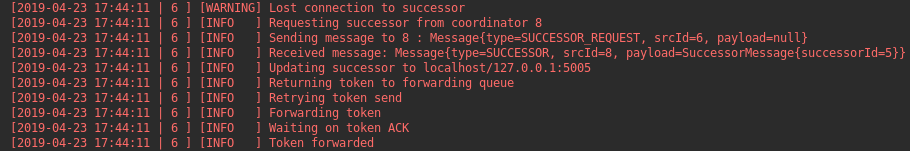
\includegraphics[width=\linewidth]{images/recovery}
	\caption{Logs from node 6 when it's successor fails to acknowledge it's sent token.}
	\label{fig:recovery}
\end{figure}

During testing, an edge case was realised with this recovery mechanism. If the disconnect is discovered when reading from the predecessor socket, there is a case where just waiting for a new predecessor does not work. Figure \ref{fig:hard} shows two scenarios where the disconnect is realised while reading from the predecessor socket. 

The scenario on the left would require A to first designate itself as its new successor before performing the self connection procedure described in the initialization protocol. This would only be necessary if the network consisted of two nodes, otherwise another node would eventually connect to A. The scenario on the right however is not one where an actual failure has occurred, and instead A is just changing its predecessor from itself to B. In order to check that the disconnect had occurred not because of failure, the token ring socket class (\emph{RingCommunicationHandler}) provided a boolean flag that would be true if the most recent disconnect had occurred while connected to itself. 

Knowing this meant that it could be assumed if there were only two nodes in the network that the other node has failed, and so a self connection would have to be performed as described in the previous section.

\begin{figure}[!ht]
	\centering
	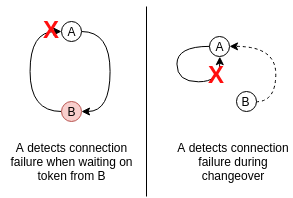
\includegraphics[width=0.6\linewidth]{images/hard}
	\caption{Two predecessor disconnect scenarios that are identical to the thread polling the predecessor socket.}
	\label{fig:hard}
\end{figure}

\subsection{Topology Persistence}

Initially, the coordinator node was always the node with the ID 6. This node would maintain an in-memory virtual representation of the network topology using a cyclic linked list of node IDs. This obviously would be useless if the coordinator was to change, and so it was necessary to persist the network topology somehow. 

This was achieved by adding a database which would behave like resource P in the practical specification (the list of nodes). Only the coordinator would be able to write and update the database, and all other nodes would read from it. The database allowed operations to be carried out as transactions, meaning that node failure during an update could be rolled back. The database is initialized using a csv file containing the ID, address, and port of each node that \emph{may} join the network at some point. Figure \ref{fig:er} shows an ER diagram of the database schema. The successorId is nullable and refers to another row in the node table. If a value is present in that column then the node ID on that row would be assumed to be part of the ring.

\begin{figure}[!ht]
	\centering
	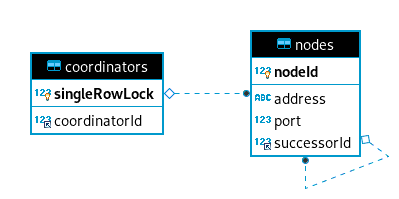
\includegraphics[width=0.6\linewidth]{images/er}
	\caption{ER diagram of the database schema for persisting the network topology.}
	\label{fig:er}
\end{figure}

When a new node wants to join the network, it first queries the database to learn who the current coordinator is. If no coordinator exists and no nodes have successors set, then this node will assume coordinator status. A limitation of this functionality is that if another node (B) queries for the current coordinator before the first node (A) has had the chance to update the database, then B could potentially also designate itself as coordinator. Since B would overwrite A as coordinator, later joining nodes would always make requests to B, and A would remain connected to itself.

The database was also essential for recovering the network topology quickly when a coordinator failed. If a node detected the failure of its successor and knew that its successor was currently the coordinator, it would temporarily act as a coordinator until a new one was elected. This would allow it to update the database and recover the ring topology by connecting to the successor of the failed coordinator. Immediately after recovering this connection, an election would be triggered by the acting coordinator in order to designate a permanent coordinator.

In order to ensure that only one coordinator existed at any time, the coordinators table included a boolean column \emph{singleRowLock} that would always be true. By setting this boolean column as the primary key, insert statements could then be constructed to either 
\begin{enumerate}
	\item Insert a new row if no coordinator exists with the value TRUE for \emph{singleRowLock}.
	\item Change the value of the coordinator ID if a row already exists by using the 'ON DUPLICATE KEY UPDATE' statement in the INSERT statement.
\end{enumerate}

Whilst another row could be added with the value FALSE for \emph{singleRowLock}, permissions would be configured such that only the hosts and a system administrator would be able to perform updates so it could be assumed that as long as the application code always used TRUE for inserts, only one row would ever exist. 

\begin{figure}[!h]
\centering
\begin{subfigure}{.5\textwidth}
  \centering
  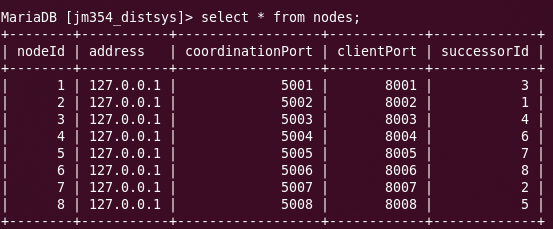
\includegraphics[width=0.95\linewidth]{images/fullring}
  \caption{Node database table.}
  \label{fig:nodetable}
\end{subfigure}%
\begin{subfigure}{.5\textwidth}
  \centering
  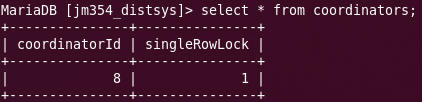
\includegraphics[width=0.95\linewidth]{images/coord}
  \caption{Coordinator database table.}
  \label{fig:coordtable}
\end{subfigure}
\caption{The state of the database after nodes join in the order 6, 5, 8, 3, 4, 7, 1, 2.}
\label{fig:dbstate}
\end{figure}

\begin{figure}[!ht]
\centering
\begin{subfigure}{.5\textwidth}
  \centering
  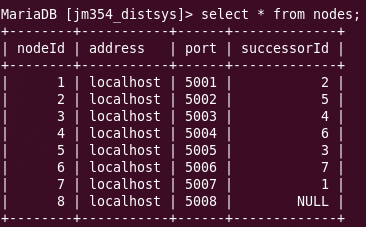
\includegraphics[width=0.95\linewidth]{images/afterfailnodes}
  \caption{Node database table.}
  \label{fig:nodetableafterfail}
\end{subfigure}%
\begin{subfigure}{.5\textwidth}
  \centering
  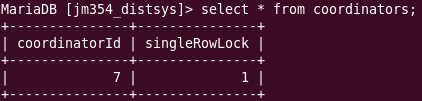
\includegraphics[width=0.95\linewidth]{images/afterfailcoord}
  \caption{Coordinator database table.}
  \label{fig:coordtableafterfail}
\end{subfigure}
\caption{The state of the database after recovering from node 8 failing.}
\label{fig:dbstateafterfail}
\end{figure}

Figure \ref{fig:dbstate} shows the state of the database after 8 nodes join in a random order. Figure \ref{fig:dbstateafterfail} shows the state of the database after node 8 fails and a new coordinator is elected.


\section{Leader/Coordinator Election}

\subsection{Election API}

An interface was used for providing a generic 'election algorithm' API, allowing different algorithms to be switched out easily. Any node.nodemessaging that arrived from either the UDP socket or the ring sockets that had the COORDINATOR\_ELECTION type would be routed to the handler for the election algorithm specified in the election header. For example, an election message that required the bully algorithm would be routed to the bully election handler.

In the configuration for each node, a default election algorithm is specified. Therefore the type of election that would be started could vary depending on which node initiated it. If a node received an election message for a different algorithm to the one they are currently using, then they would replace their election handler with one that could process the arriving message. 

The methods required by the election API are summarised in table \ref{tbl:elecapi}. The constructors could vary since different resources may be necessary. For example, the ring-based and Chang Roberts algorithms both only require communication around the ring, whilst the Bully algorithm only requires communication across the ring.

\begin{table}[!ht]
\centering
\resizebox{\textwidth}{!}{%
\begin{tabular}{ll}
\hline
Method                                 & Usage                                                                                      \\ \hline
\multicolumn{1}{l|}{getMethodName}     & Returns the name of the underlying algorithm used by the implementation of this interface. \\
\multicolumn{1}{l|}{startElection}     & Starts an election.                                                                        \\
\multicolumn{1}{l|}{handleMessage}     & Handles any election node.nodemessaging.                                                             \\
\multicolumn{1}{l|}{getResult}         & Returns the result of the election (if concluded).                                         \\
\multicolumn{1}{l|}{electionConcluded} & Returns true if a result has been obtained.                                                \\ \hline
\end{tabular}%
}
\caption{Methods of the election handler interface.}
\label{tbl:elecapi}
\end{table}

\subsection{Triggering Elections}

Initially, elections could only be triggered by the predecessor of a failed coordinator. This meant that if a new node joined with a higher ID, it would not be elected until the current coordinator failed. This was resolved by adding logic to the joining procedure that once part of the ring, the new node would trigger an election if it found that its ID was greater than the current coordinators. 

This meant it would be possible for multiple elections to be ongoing simultaneously if many nodes joined the ring in quick succession with higher IDs than the current coordinator. 

\subsection{Ring-Based}

The ring based algorithm was the simplest to implement and test. The node starting the election would initialise the ELECTION message with its own ID and forward this to its successor and set the \emph{ongoing} flag to true. The message would be forwarded around the ring by each node after appending their ID to the list of candidates until it returned to the node that started the election. 

This node then chose the new coordinator from the list of candidates based on which had the highest ID, and forwarded the result to its successors as a COORDINATOR message. The result would be forwarded by each node until it reached a node that was already aware of the new coordinator.

\begin{figure}[!ht]
	\centering
	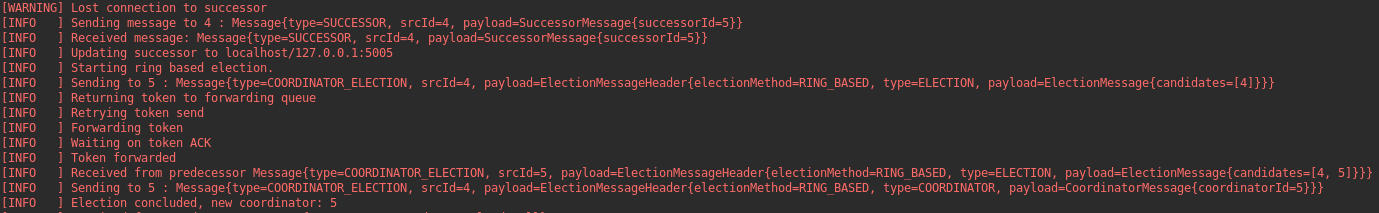
\includegraphics[width=\linewidth]{images/ringelec}
	\caption{Logs from node 2 after detecting coordinator failure. Note how token passing resumes as soon as a new successor is found despite the loss of the coordinator in order to make node failure transparent.}
	\label{fig:ringbased}
\end{figure}

\subsection{Chang Roberts}

The Chang Roberts algorithm reused most of the components from the ring-based algorithm, other than the forwarding logic for ELECTION node.nodemessaging.

If the ELECTION message contained the receiving nodes ID, then it would conclude the election and forward the COORDINATOR message as in the ring-based algorithm. However, in order to avoid redundant forwarding of election node.nodemessaging if two elections are started at the same time, ELECTION node.nodemessaging would only be forwarded if the receiving node was a better candidate (i.e. had a greater ID), or if it had not already participated by forwarding a message previously.

Figure \ref{fig:chang} shows logs from a new node that has joined the ring and triggered an election. Initially the election message is sent, and later it returns with the same ID and so node 8 elects itself. It then forwards the coordinator message until it arrives back to itself at which point it is dropped.

\begin{figure}[!ht]
	\centering
	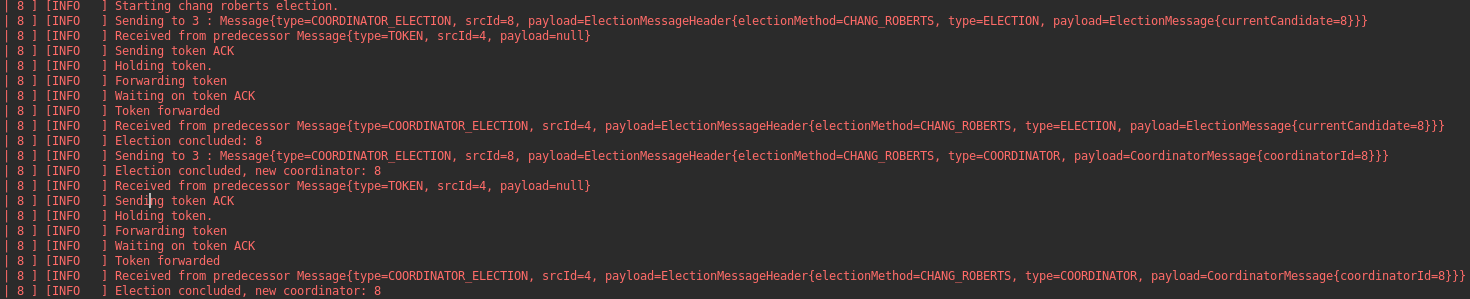
\includegraphics[width=\linewidth]{images/chang}
	\caption{Logs from node 8 when it joins the ring and notices its ID is greater than the current coordinator.}
	\label{fig:chang}
\end{figure}

\subsection{Bully}

The bully algorithm was the most difficult to implement due to its dependence on timing. An election would be started by a node by sending an ELECTION message to all nodes with IDs greater than it's own. It would then create a thread which would sleep for a preset time before assuming it is to be the coordinator. If one of the other nodes that received the ELECTION message replied with an OK message, the sleeping thread would simply terminate after the preset time had expired. Another thread would be spawned to again sleep for a duration of time after receiving the OK message. If no coordinator message was received before this second duration elapsed, then the node would restart the election.

Each node that received an ELECTION message would reply with an OK message if it had not already started an election, and then carry out the same procedure as the first node had to trigger the election. Eventually the node with the highest ID would not have any other nodes to send ELECTION node.nodemessaging to, and so it would consider itself the coordinator and inform all the other nodes in the ring using the COORDINATOR message.

Figure \ref{fig:bully} shows how effective the bully algorithm is at dealing with failure and demonstrates a node being bullied into letting another node be coordinator. The order of events in the logs shown are:

\begin{enumerate}
	\item Node 6 receives election message from node 4.
	\item 6 replies with OK message, and begins its own election by sending an election message to node 7.
	\item 6 also receives election message from node 5, but ignores it since it is already carrying out an election.
	\item Timeout occurs without 7 sending OK message, 6 tries to elect self as coordinator and sends coordinator message to all other nodes.
	\item Node 7 has in the meantime elected itself as coordinator, and 'bullies' node 6 into letting it be coordinator.
\end{enumerate}

\begin{figure}[!ht]
	\centering
	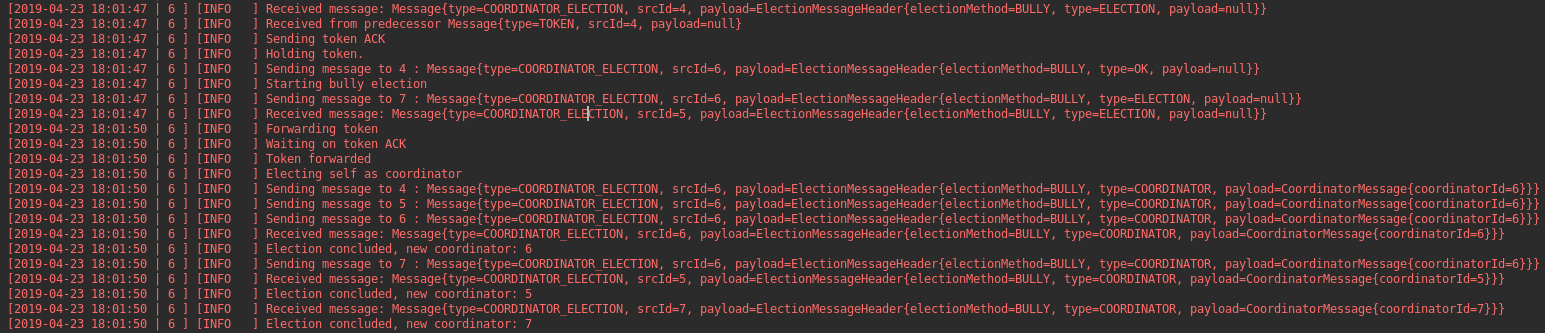
\includegraphics[width=\linewidth]{images/bully}
	\caption{Logs from node 6 during an election where coordinator 8 has failed, and 7 should be the next coordinator.}
	\label{fig:bully}
\end{figure}

\section{Receive/Send Posts}

\subsection{Mutual Exclusion}

At any one time, only one server/node should be able to read or write from the message queue. In order to provide this mutual exclusion, the token-ring method was used. A token is created by the first node in the ring when initializing the network, and is forwarded around the ring after a) the node holding the token carries out a operation on the resource or b) a timeout expires. 

Since only one node can have the token at any one time, mutual exclusion is ensured. No starvation can occur since the token will always eventually return to each node in the ring. The downsides of the token-ring algorithm is that the wait time between each operation grows linearly with the size of the ring. It also requires some sort of recovery mechanism if the node holding the token fails.

In order to ensure that the token is at least delivered successfully, the token acknowledgement message described earlier for detecting lost nodes was utilised. The following steps are taken between waiting on a token and forwarding it:

\begin{enumerate}
	\item Ring message handling thread polls predecessor socket for token.
	\item Client handling thread polls the single element \emph{usableTokenQueue} waiting for the token to become available.
	\item When the token arrives, the ring message thread replies with an ACK, and puts the token in the \emph{usableTokenQueue} for the client thread to consume. It then begins polling the single element \emph{forwardableTokenQueue} where the client thread will return the token.
	\item The client thread dequeues the token from the \emph{usableTokenQueue} and uses it to serve it's clients then returns it to ring thread via the \emph{forwardableTokenQueue}.
	\item Ring thread then removes the token from the \emph{forwardableTokenQueue} and forwards it onto it's successor.
\end{enumerate}

\subsection{Server}

In order for each node in the ring to serve clients, they each provide a TCP server socket. In order to isolate coordination traffic from client traffic, clients used a different port to connect to the node than other nodes. To allow for local testing, it was necessary to use port numbers to differentiate between host sockets on the same machine. In a realistic scenario, each node would have a different host address (and even a different FQDN) and a consistent port for client traffic and coordination traffic. 

I had hoped to use an existing protocol such as Websockets so that the client-to-server communication followed some standard. Due to time constraints however, I opted for simply sending messages over the TCP socket, using line breaks to seperate each message. This time I serialized the messages to JSON to allow any application to consume and communicate with the server as a client, in contrast to the direct serialization of POJOs which is used for communication between nodes.

The web server consisted of a fixed size thread pool for serving up to two clients. A server socket would would wait for a client to connect, and then spin up a client handler thread for processing the new client. Clients and servers would send messages as JSON, using a newline (\lstinline{\n}) as a delimiter for messages. Each JSON object sent included a \emph{messageType} field with one of the values in table \ref{tbl:clientmessagetypes}. JSON encoding and decoding was performed using the Gson library. 

A publish-subscribe pattern was used for communication. Clients would send a log in message with a username so that the server knew which messages to send their way. They could also join groups would allow for messages to be broadcast to multiple clients. 

\begin{table}[!h]
\centering
\resizebox{\textwidth}{!}{%
\begin{tabular}{@{}lll@{}}
\toprule
Message Type                               & Usage                                                                                                                        & Payload                  \\ \midrule
\multicolumn{1}{l|}{LOGIN}                  & \multicolumn{1}{l|}{Sent by client to declare a username to the node.}                                              & Username \\
\multicolumn{1}{l|}{JOIN\_GROUP}             & \multicolumn{1}{l|}{Sent by client to subscribe to a group.}                                     & Name of group to join.\\
\multicolumn{1}{l|}{LEAVE\_GROUP}    & \multicolumn{1}{l|}{Sent by client to unsubscribe from a group.} & Name of group to leave.\\
\multicolumn{1}{l|}{CHAT\_MESSAGE}                 & \multicolumn{1}{l|}{Text sent between clients.}                                                                        & To, From, Time, Contents \\
\multicolumn{1}{l|}{ERROR}            & \multicolumn{1}{l|}{Sent by server if an error occurs}                   & Explanation \\ \bottomrule
\end{tabular}%
}
\caption{Messages sent between client and server.}
\label{tbl:clientmessagetypes}
\end{table}

\subsection{Client}

\section{Testing}

\section{Evaluation}

\section{Summary}

\section{How to Run}

\bibliographystyle{unsrt}
\bibliography{mybib}

\end{document}
